\documentclass[14pt, a4paper]{article}
\usepackage[russian]{babel}
\usepackage{graphicx}
\usepackage{layout}

\usepackage[14pt]{extsizes}

\setcounter{tocdepth}{4}
\setcounter{secnumdepth}{4}

\usepackage{xcolor}
\usepackage{hyperref}

\usepackage{listings}

 % Цвета для гиперссылок
\definecolor{linkcolor}{HTML}{000000} % цвет ссылок
\definecolor{urlcolor}{HTML}{000000} %цвет гиперссылок

\hypersetup{pdfstartview=FitH,  linkcolor=linkcolor,urlcolor=urlcolor, colorlinks=true}

\definecolor{codegreen}{rgb}{0,0.6,0}
\definecolor{codegray}{rgb}{0.5,0.5,0.5}
\definecolor{codepurple}{rgb}{0.58,0,0.82}
\definecolor{backcolour}{rgb}{0.97,0.97,0.97}

%таблица
\lstdefinestyle{mystyle}{
    backgroundcolor=\color{backcolour},   
    commentstyle=\color{codegreen},
    keywordstyle=\color{magenta},
    numberstyle=\tiny\color{codegray},
    stringstyle=\color{codepurple},
    basicstyle=\ttfamily\footnotesize,
    breakatwhitespace=false,         
    breaklines=true,                 
    captionpos=b,                    
    keepspaces=true,
    frame=single,                                                    
    showspaces=false,                
    showstringspaces=false,
    showtabs=false,                  
    tabsize=2,
    mathescape=true
}

\lstset{style=mystyle, extendedchars=\true, literate=
{а}{ {\selectfont\char224} }1
{б}{ {\selectfont\char225} }1
{в}{ {\selectfont\char226} }1
{г}{ {\selectfont\char227} }1
{д}{ {\selectfont\char228} }1
{е}{ {\selectfont\char229} }1
{ё}{ {\"e} }1
{ж}{ {\selectfont\char230} }1
{з}{ {\selectfont\char231} }1
{и}{ {\selectfont\char232} }1
{й}{ {\selectfont\char233} }1
{к}{ {\selectfont\char234} }1
{л}{ {\selectfont\char235} }1
{м}{ {\selectfont\char236} }1
{н}{ {\selectfont\char237} }1
{о}{ {\selectfont\char238} }1
{п}{ {\selectfont\char239} }1
{р}{ {\selectfont\char240} }1
{с}{ {\selectfont\char241} }1
{т}{ {\selectfont\char242} }1
{у}{ {\selectfont\char243} }1
{ф}{ {\selectfont\char244} }1
{х}{ {\selectfont\char245} }1
{ц}{ {\selectfont\char246} }1
{ч}{ {\selectfont\char247} }1
{ш}{ {\selectfont\char248} }1
{щ}{ {\selectfont\char249} }1
{ъ}{ {\selectfont\char250} }1
{ы}{ {\selectfont\char251} }1
{ь}{ {\selectfont\char252} }1
{э}{ {\selectfont\char253} }1
{ю}{ {\selectfont\char254} }1
{я}{ {\selectfont\char255} }1
{А}{ {\selectfont\char192} }1
{Б}{ {\selectfont\char193} }1
{В}{ {\selectfont\char194} }1
{Г}{ {\selectfont\char195} }1
{Д}{ {\selectfont\char196} }1
{Е}{ {\selectfont\char197} }1
{Ё}{ {\"E} }1
{Ж}{ {\selectfont\char198} }1
{З}{ {\selectfont\char199} }1
{И}{ {\selectfont\char200} }1
{Й}{ {\selectfont\char201} }1
{К}{ {\selectfont\char202} }1
{Л}{ {\selectfont\char203} }1
{М}{ {\selectfont\char204} }1
{Н}{ {\selectfont\char205} }1
{О}{ {\selectfont\char206} }1
{П}{ {\selectfont\char207} }1
{Р}{ {\selectfont\char208} }1
{С}{ {\selectfont\char209} }1
{Т}{ {\selectfont\char210} }1
{У}{ {\selectfont\char211} }1
{Ф}{ {\selectfont\char212} }1
{Х}{ {\selectfont\char213} }1
{Ц}{ {\selectfont\char214} }1
{Ч}{ {\selectfont\char215} }1
{Ш}{ {\selectfont\char216} }1
{Щ}{ {\selectfont\char217} }1
{Ъ}{ {\selectfont\char218} }1
{Ы}{ {\selectfont\char219} }1
{Ь}{ {\selectfont\char220} }1
{Э}{ {\selectfont\char221} }1
{Ю}{ {\selectfont\char222} }1
{Я}{ {\selectfont\char223} }1
}

\lstset{style=mystyle}

%Разметка страницы
\oddsidemargin = 0pt
\marginparwidth = 45pt 
\textwidth = 467pt
\textheight = 716pt
\topmargin = 0pt 
\footskip = 30pt 
\headheight = 0pt 
\headsep = 0pt 

\begin{document}
\begin{titlepage}
    \topmargin=216pt
    \newpage
    \hangindent=0.7cm
    \huge ИУ-10\\
    Системное\\
    Программное\\
    Обеспечение\\
    Системы виртуализации\\
    \textbf{Системы
    управления\\
    виртуализацией}

    \vspace{9cm}

    \begin{center}
        \small\textit{Москва, 2022}
    \end{center}
\end{titlepage}

\section*{На этом уроке}
\begin{enumerate}
    \item Рассмотрим роль системы управления виртуализацией, механизмы развёртывания и
    масштабирования гостевых систем.
    \item Разберём примеры широко используемых на практике систем управления: VMware vCenter
    Server, Proxmox, oVirt.
    \item Создадим настольную лабораторию с Proxmox.
\end{enumerate} 

\tableofcontents 
\newpage

\section*{Роль системы управления виртуализацией} 
\addcontentsline{toc}{section}{Роль системы управления виртуализацией}

Ранее мы говорили о самых разнообразных системах виртуализации, начиная с персональных
виртуальных машин, заканчивая контейнерами систем и приложений. В первую очередь мы
рассматривали каждый экземпляр гипервизора или даже хозяйской системы с гипервизором
виртуальной машины в отдельности. Такой подход вполне уместен при исследовании виртуальных
машин или индивидуальном их использовании для решения не слишком сложных задач.\\

Самые очевидные применения:

\begin{enumerate}
    \item Эмуляция физической машины с архитектурой или операционной системой, отличной от той,
    что есть на хозяйской системе. Так мы можем запускать ПО, отсутствующее на хозяйской
    системе.
    \item Создание ещё одной машины. Так мы можем поэкспериментировать с настройками ОС
    гостевой системы, его ПО и т. д. Или запустить на такой «чистой» системе какие-то службы и
    не переживать по поводу совместимости различных служб, одновременно запущенных на
    одной машине.
\end{enumerate}

Однако существуют задачи, для решения которых одной виртуальной машины или даже одного
гипервизора недостаточно. В частности:

\begin{enumerate}
    \item Требуемая вычислительная мощность системы превышает мощность любой отдельно взятой
    физической машины. Решение состоит в использовании кластера вычислительных машин с
    распределением нагрузки по отдельным машинам.
    \item Необходимо масштабировать доступные вычислительные ресурсы, необходимость в которых
    меняется со временем. Это позволяет достигать более высокой эффективности
    использования оборудования.
    \item Необходимо обеспечить высочайшую надёжность всей системы в целом. Тогда речь заходит о
    резервировании машин с возможностью переключения между машинами в режиме реального
    времени практически без остановки основной работы. В данном случае обычно говорят об
    обеспечении высокой доступности системы (High Availability) и отказоустойчивости (Fault
    tolerance).
\end{enumerate}

Всё это возможно при использовании кластера машин, однако ручное управление кластером — не
самое удачное решение. Живому существу сложно уследить за сотнями машин, контролируя
множество параметров: состояние машин, их загруженность вычислениями, данными и т. д. А потому
для управления кластерами машин и, в частности, виртуальных машин были созданы специальные
программные комплекты — системы управления виртуализацией.

\subsection*{Сохранение состояния виртуальной машины (snapshot)} 
\addcontentsline{toc}{subsection}{Сохранение состояния виртуальной машины (snapshot)}

\begin{figure}[h]
    \centering
    \scalebox{0.9}{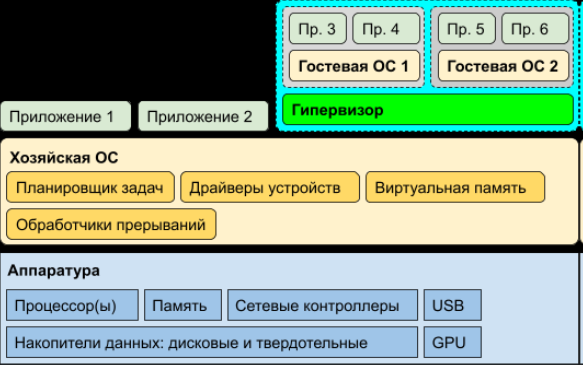
\includegraphics[width=1\textwidth]{1.png}}\\ 
    \small\textit{Создание снимка ВМ}  
    \label{framework} 
\end{figure}

В некоторых ситуациях бывает очень полезно и удобно зафиксировать и сохранить полное текущее
состояние ВМ — сделать снимок (snapshot) ВМ. Типичный пример применения снимка — обновление
ОС внутри ВМ. Если обновление приведёт к некорректной работе ВМ, при наличии снимка
предыдущего состояния можно просто вернуться к нему и продолжать работу, пока ответственные за
обновление инженеры не разберутся с проблемой. Однако ввиду простоты использования и
кажущихся достоинств \href{https://www.vmgu.ru/news/vmware-vsphere-esx-snapshots-are-bad}{снимки зачастую используют не по назначению}. Например, как средство
резервного копирования ВМ. Тем не менее системы управления виртуализацией обычно
предоставляют средства централизованного и удалённого управления снимками ВМ, что, разумеется,
упрощает жизнь системным администраторам.

\subsection*{Создание клонов и развёртывание гостевых систем из
шаблонов} 
\addcontentsline{toc}{subsection}{Создание клонов и развёртывание гостевых систем из
шаблонов}

Если вычислительную задачу или оказываемый сервис можно разделить на несколько выполняемых
параллельно задач, то можно повысить вычислительную мощность системы в целом, добавив
исполнительных устройств. Другими словами, если можно использовать ещё N физических серверов
и на них запустить ещё по M виртуальных машин, то можно увеличить количество используемых в
системе ВМ на N * M. Выглядит весьма привлекательно. Самое простое решение состоит в создании
максимально полных копий одной из существующих ВМ — клонов. Клоном называется копия
остановленной ВМ. Из выполняющейся в данный момент ВМ возможно только создание снимков
(snapshot).


\begin{figure}[h]
    \centering
    \scalebox{0.9}{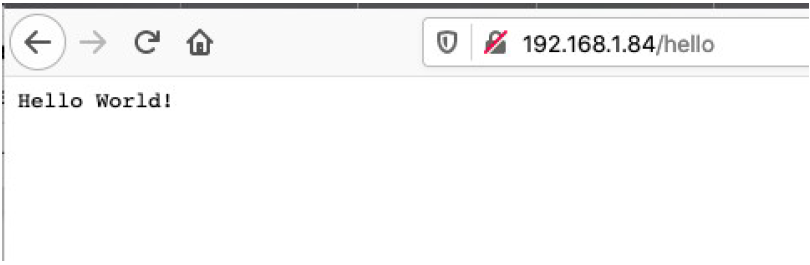
\includegraphics[width=1\textwidth]{2.png}}\\ 
    \small\textit{Создание клона ВМ из ВМ со снимками}  
    \label{framework} 
\end{figure}

К сожалению, такой подход имеет недостатки. В частности, если сохранить все свойства исходной
ВМ, то в системе возникнут коллизии, связанные с существованием двух идентичных ВМ. При
наличии двух ВМ с одинаковыми MAC-адресами сетевых интерфейсов будет невозможна корректная
маршрутизация сетевых пакетов. Также система управления ВМ не сможет корректно управлять
двумя ВМ с одинаковыми идентификаторами. Чтобы избежать этих проблем, системы управления ВМ
вносят необходимые изменения в настройки клонов.

\begin{figure}[h]
    \centering
    \scalebox{0.9}{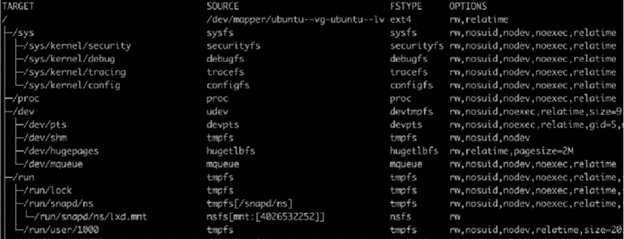
\includegraphics[width=1\textwidth]{3.png}}\\ 
    \small\textit{Создание шаблона и новых ВМ из шаблона}  
    \label{framework} 
\end{figure}

Другой часто используемый способ заключается в создании шаблона — предварительно настроенной
ВМ, переведённой в особое состояние, когда её запуск и любые модификации запрещены. Этот
запрет предохраняет шаблон от непреднамеренного запуска и изменения. При необходимости внести
изменения в шаблон он переводится в состояние ВМ, модифицируется и снова преобразуется в
шаблон.

\subsection*{Живая миграция и масштабирование} 
\addcontentsline{toc}{subsection}{Живая миграция и масштабирование}

\begin{figure}[h]
    \centering
    \scalebox{0.9}{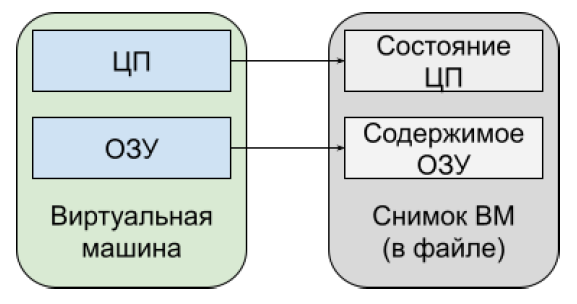
\includegraphics[width=1\textwidth]{4.png}}\\ 
    \small\textit{VMware vSphere vMotion}  
    \label{framework} 
\end{figure}

Итак, мы знаем, как создать дополнительные виртуальные машины из шаблона или из уже
имеющейся ВМ. Следующая задача — запуск новой виртуальной машины, чтобы она наконец-то
начала выполнять полезную работу. Имея возможность запускать создаваемые ВМ только на одном
физическом сервере, мы достаточно быстро исчерпаем его вычислительные ресурсы. Дальнейшее
добавление новых ВМ будет приводить к существенной деградации производительности уже
запущенных ВМ. Очевидно, решение проблемы состоит в запуске ВМ на дополнительных серверах.
Но это должны быть не изолированные друг от друга машины, а связанные друг с другом системы,
управляемые специальным программным обеспечением, о котором мы будем говорить дальше. Если
не вдаваться в технические детали, обсуждаемое ПО совместно с гипервизором должно решать
следующие задачи:

\begin{enumerate}
    \item Создание новых ВМ при недостаточной производительности совокупности уже имеющихся.
    \item Уничтожение имеющихся ВМ, если нагрузка на систему в целом существенно превышает
    мощности запущенных ВМ.
    \item Перенос ВМ с одного физического сервера на другой в целях балансировки нагрузки.
\end{enumerate}

Важно отметить, что перенос ВМ с одного сервера на другой происходит практически незаметно.
\vspace{0.3cm}
\begin{lstlisting}
$\textdollar$ ping 192.168.122.88
64 bytes from 192.168.122.88: icmp_seq=637 ttl=64 time=1.00 ms
64 bytes from 192.168.122.88: icmp_seq=638 ttl=64 time=0.570 ms
64 bytes from 192.168.122.88: icmp_seq=639 ttl=64 time=0.473 ms
64 bytes from 192.168.122.88: icmp_seq=640 ttl=64 time=0.529 ms
64 bytes from 192.168.122.88: icmp_seq=641 ttl=64 time=5.35 ms <- Миграция 
64 bytes from 192.168.122.88: icmp_seq=643 ttl=64 time=0.455 ms
64 bytes from 192.168.122.88: icmp_seq=644 ttl=64 time=0.255 ms
64 bytes from 192.168.122.88: icmp_seq=645 ttl=64 time=0.417 ms
\end{lstlisting}

\subsection*{Высокая доступность} 
\addcontentsline{toc}{subsection}{Высокая доступность}

\begin{figure}[h]
    \centering
    \scalebox{0.9}{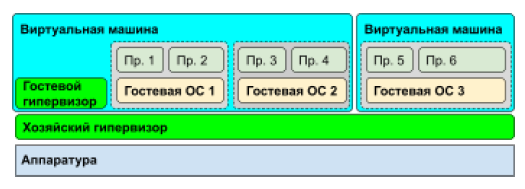
\includegraphics[width=1\textwidth]{5.png}}\\ 
    \small\textit{VMware vCenter server high availability}  
    \label{framework} 
\end{figure}

Безусловно, плановое управление совокупной вычислительной мощностью системы — это основная
задача системы управления виртуализацией. Однако иногда случаются разные неприятности:

\begin{itemize}
    \item оборудование (сервер, сетевые маршрутизаторы, блоки питания) может выйти из строя;
    \item провода, соединяющие серверы, могут быть повреждены беспечным обслуживающим
    персоналом;
    \item комбинация ПО, состоящая из гипервизора, ОС и ПО гостевой системы, может привести к
    краху сервера и последующей его неработоспособности или как минимум перезагрузке.
\end{itemize}

Судя по статистике, собранной при использовании реальных центров обработки данных, подобные
ситуации вполне имеют место. Для минимизации последствий используются специальные методики,
повышающие доступность вычислительной системы в целом, то есть делающие системы
высокодоступными (от англ. Highly Available).\\

Для понимания серьёзности ситуации интересно сопоставить процент времени, проводимого
системой в работоспособном состоянии, с временем недоступности системы. Например, в
соответствии с исследованием 32 хостинг-провайдеров в течение 2018 года среднее значение
доступности составило 99,59\%, что соответствует 35,5 часам в год. Хотя многие хостинги обещают
99,99\%, что дало бы время простоя примерно 53 минуты в год. Полную статистику можно посмотреть
в статье \href{https://hostingfacts.com/average-hosting-uptime-study/}{Average Web Hosting Uptime in 2018 For 32 Hosts}.\\

Когда говорят о высокой доступности виртуальных машин, обычно речь идёт об автоматическом
перезапуске виртуальной машины на работающем сервере, если ранее используемый сервер вышел
из строя или даже стал недоступен из-за, например, проблем с сетевым подключением. Причём
перезапуск ВМ на новом сервере — это не единственная проблема в данном случае. Перед
перезапуском ВМ необходимо сначала обнаружить ситуацию выхода из строя одного или нескольких
серверов кластера, затем позаботиться о том, чтобы выбывшие сервера не навредили пока ещё
работоспособным своими неожиданными действиями, и только затем перезапускать ВМ.\\

Важная особенность, связанная с обнаружением выбывших машин: группы машин кластера могут
потерять связь друг с другом (то есть группа с группой), но внутри группы связь между машинами
может быть сохранена, равно как как и связь с «внешним миром». В таком случае каждая из групп
может принять решение работать самостоятельно. Эта ситуация называется split brain. По-видимому,
в настоящее время нет устоявшегося перевода данного термина относительно виртуальных машин
и/или вычислительных кластеров. Но можно предположить, что подходящим по смыслу вариантом
могло бы быть «раздвоение личности» или «раздвоение/расщепление сознания».\\

Чтобы такие ситуации не возникали, существует договорённость о том, что только группа машин,
составляющая кворум, продолжает нормальное функционирование, а также предпринимает попытку
отключить или заблокировать вторую группу машин.\\

\href{https://ru.wikipedia.org/wiki/Кворум}{\underbar{Кворум}} (лат. quorum praesentia sufficit — «которых присутствие достаточно») — установленное
законом, уставом организации или регламентом число участников собрания (заседания), достаточное
для признания данного собрания правомочным принимать решения по вопросам его повестки дня.\\

Машины вне кворума должны добровольно остановить свою работу. Процесс изоляции машин вне
группы кворума называется \href{https://en.wikipedia.org/wiki/Fencing_(computing).}{\underbar{ограждением}} (от англ. fencing). В англоязычной литературе также
используются акронимы STONITH (Shoot The Other Node In The Head — «стреляй другому узлу в
голову») или STOMITH (Shoot The Other Machine In The Head — «стреляй другой машине в голову»). В
любом случае подразумевается максимально жёсткий метод вывода из строя узлов, то есть серверов,
оказавшихся вне кворума. В серьёзных центрах обработки данных отключение серверов происходит
путём отключения их от питания благодаря управляемым источникам питания. В более простых
случаях используется отключение сетевых соединений на управляемых сетевых маршрутизаторах.
Самый простой вариант — использование сторожевых таймеров на самих машинах, которые,
например, зависли, выполняя некоторый набор ПО.\\

Именно поэтому не рекомендуют даже в исследовательских целях использовать кластеры, состоящие
всего из двух узлов. При потере связи между узлами кворума быть не может, потому что каждый будет
считать себя кворумом с одинаковой на то мотивацией.\\

Справедливости ради стоит отметить, что и при наличии всего двух узлов можно реализовать кворум.
Для этого обычно используют ещё один независимый сетевой накопитель данных. Идея в том, что
если целостность сети в целом не нарушена и только один из узлов потерял доступ к сети, второй
узел всё ещё может получить доступ к независимому сетевому накопителю, а потому совместно с
этим сетевым накопителем считается кворумом.\\

При реализации кластеров с высокой доступностью важно иметь в виду следующие аспекты:

\begin{enumerate}
    \item Данные, с которыми происходит работа, и сама операционная система, используемая в ВМ,
    должны храниться на общедоступном ресурсе. То есть не на локальном диске данного
    сервера, а на сетевом накопителе. В таком случае выход из строя одного из узлов приводит
    лишь к потере временных данных, которые ещё не были сохранены на общем накопителе.
    \item Содержимое памяти узла, так или иначе покинувшего кворум, оказывается навсегда утеряно.
    \item Восстановление ВМ на другом узле занимает время, складывающееся из времени принятия
    решения о недоступности узла или группы узлов, времени загрузки целевой ВМ и старта на
    ней необходимых сервисов. Речь, как правило, идёт о десятках секунд или даже минутах.
\end{enumerate}

\begin{lstlisting}
$\textdollar$ ping 192.168.122.188
64 bytes from 192.168.122.188: icmp_seq=25 ttl=64 time=0.811 ms
64 bytes from 192.168.122.188: icmp_seq=26 ttl=64 time=0.355 ms
From 192.168.122.1 icmp_seq=58 Destination Host Unreachable
From 192.168.122.1 icmp_seq=59 Destination Host Unreachable

... Отключение ВМ ...

From 192.168.122.1 icmp_seq=197 Destination Host Unreachable
From 192.168.122.1 icmp_seq=198 Destination Host Unreachable

64 bytes from 192.168.122.188: icmp_seq=202 ttl=64 time=0.458 ms
64 bytes from 192.168.122.188: icmp_seq=203 ttl=64 time=0.290 ms
64 bytes from 192.168.122.188: icmp_seq=204 ttl=64 time=0.413 ms
\end{lstlisting}

\subsection*{Отказоустойчивость} 
\addcontentsline{toc}{subsection}{Отказоустойчивость}

\begin{figure}[h]
    \centering
    \scalebox{0.9}{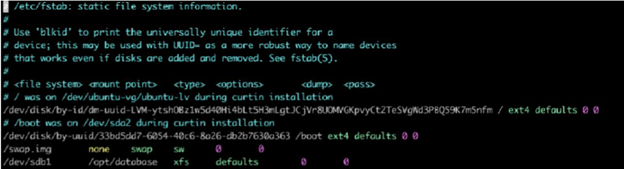
\includegraphics[width=1\textwidth]{6.png}}\\  
    \label{framework} 
\end{figure}

Если минуты или даже секунды простоя хотя бы одной ВМ неприемлемы, то используются несколько
другие механизмы. По сути, в данном случае речь идёт о перманентной живой миграции с основной
ВМ на первом сервере в теневую ВМ на другом. Как только сервер с одной из «мигрируемых» ВМ
оказывается недоступен, исполнение продолжает оставшаяся ВМ, и ей тут же находится другая
теневая копия. Такой подход позволяет сохранить даже содержимое памяти ВМ, но, к сожалению,
устанавливает довольно жёсткие требования к оборудованию и окружению.\\

VMware Fault Tolerance — одна из наиболее известных систем такого рода. Возможно, это
единственная реально рабочая система. Она имеет следующие \href{https://docs.vmware.com/en/VMware-vSphere/6.7/com.vmware.vsphere.avail.doc/GUID-57929CF0-DA9B-407A-BF2E-E7B72708D825.html}{требования и ограничения}:

\begin{enumerate}
    \item Требования:
    \begin{enumerate}
        \item[a.] Как минимум 10-гигабитное сетевое соединение с низкими задержками.
        Предпочтительно выделенное соединение между серверами, участвующими в
        реализации Fault Tolerance.
        \item[b.] Процессоры с аппаратной поддержкой виртуализации MMU: Intel семейства Sandy
        Bridge и более поздние, AMD семейства Bulldozer и более поздние.
    \end{enumerate}
    \item Ограничения, действующие независимо друг от друга:
    \begin{enumerate}
        \item[a.] Максимальное число защищённых механизмом Fault Tolerance ВМ на одном сервере
        — не более четырёх.
        \item[b.] Максимальное число защищённых механизмом Fault Tolerance vCPU (виртуальных
        процессоров) на одном сервере — не более восьми. Например, можно представить
        себе четыре защищённые ВМ, каждой из которых выделено по два vCPU.
    \end{enumerate}
\end{enumerate}

Из-за этих ограничений системы сложно и дорого масштабировать. А ещё возникает вопрос, какова
реальная производительность такого решения. Можно ожидать, что она будет несколько ниже по
сравнению с ВМ, запущенными в обычном режиме.\\

Судя по тому, что никаких других решений подобного рода, кроме VMware Fault Tolerance, в данный
момент не существует на рынке, есть подозрение, что спрос на них не так уж и велик. То есть, видимо,
все предпочитают более простую и дешёвую реализацию High Availability. Ранее существовала
\href{https://wiki.xenproject.org/wiki/Remus}{надстройка для Xen под названием Remus}, но о ней ничего не слышно в последние несколько лет.
Думается, что проект был заброшен за ненадобностью.

\section*{Примеры реализации} 
\addcontentsline{toc}{section}{Примеры реализации}

\subsection*{VMware vCenter Server} 
\addcontentsline{toc}{subsection}{VMware vCenter Server}

Будучи пионером современных систем виртуализации, компания VMware, разумеется, достаточно
давно разработала и стала предлагать своим клиентам решение для управления кластером
виртуальных машин. Это VMware vCenter Server, ранее именовавшийся VMware VirtualCenter.
Интересно, что в настоящее время VMware vCenter Server распространяется только как appliance, то
есть образ отдельной виртуальной машины. VMware vSphere версии 6.7 был последним продуктом, с
которым распространялся VMware vCenter Server как отдельное приложение для Microsoft Windows.\\

Тем не менее VMware vCenter Server — это важнейший компонент виртуализованной
инфраструктуры, позволяющий управлять как отдельными виртуальными машинами, так и кластером
виртуальных машин, задавая режимы работы кластера.\\

\begin{figure}[h]
    \centering
    \scalebox{0.75}{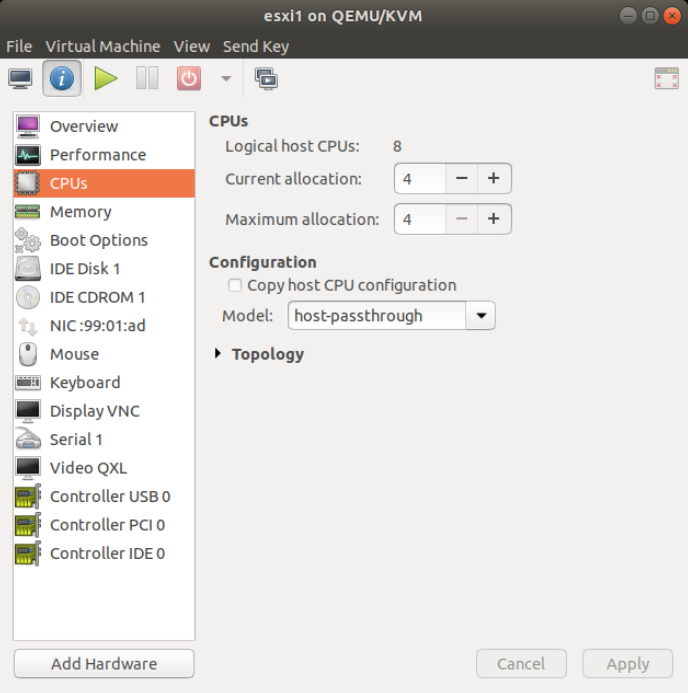
\includegraphics[width=1\textwidth]{7.png}}\\ 
    \small\textit{Модель кластера из виртуальных машин поверх гипервизора VMware ESXi под управлением VMware vCenter
    Server, \href{https://docs.vmware.com/en/VMware-vSphere/index.html}{VMware vSphere Documentation}}  
    \label{framework} 
\end{figure}

\newpage

\begin{figure}[h]
    \centering
    \scalebox{0.5}{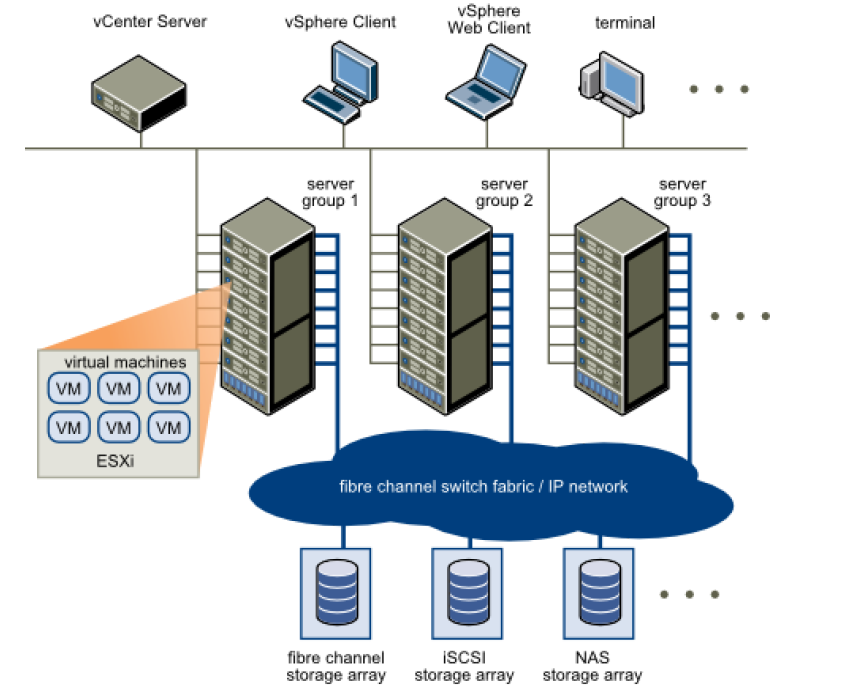
\includegraphics[width=1\textwidth]{8.png}}\\ 
    \small\textit{Физическая топология центра обработки данных на базе инфраструктуры VMware,
    \href{https://docs.vmware.com/en/VMware-vSphere/index.html}{vSphere Concepts and Features}.}  
    \label{framework} 
\end{figure}

\href{https://www.vmware.com/content/dam/digitalmarketing/vmware/ru/pdf/products/vCenter/vmw-datasheetvcenter.pdf}{VMware vCenter} обладает следующими возможностями:
\begin{enumerate}
    \item Клиент vSphere на основе HTML5.
    \item vCenter Single Sign-on: упрощение администрирования благодаря возможности выполнить
    вход в систему один раз и обращаться ко всем экземплярам vCenter без повторной проверки
    подлинности.
    \item Оповещения и уведомления: поддержка новых объектов, показателей и событий, таких как
    оповещения, связанные с определённым хранилищем данных и виртуальной машиной. Эти
    оповещения могут запускать новые автоматизированные рабочие процессы для устранения
    проблем и предотвращения их возникновения.
    \item Встроенные средства резервного копирования и восстановления: готовое решение по
    резервному копированию на уровне файлов с удобным пользовательским интерфейсом. Оно
    устраняет необходимость в сторонних средствах резервного копирования для защиты
    серверов vCenter и контроллеров Platform Services Controller (PSC).
    \item Средство планирования резервного копирования и восстановления: планирование резервного
    копирования vCenter Server Appliance и управление количеством хранимых резервных копий.
    Использование API-интерфейсов REST для упрощения резервного копирования и
    восстановления.
    \item vCenter Server High Availability: защита vCenter Server Appliance и связанных служб благодаря
    встроенной поддержке высокой доступности и целевому времени восстановления менее
    десяти минут.
    \item Профили узлов: стандартизация и упрощение управления конфигурациями узлов VMware
    ESXi. Сохранение схемы проверенной конфигурации, включающей в себя параметры сети,
    хранилища и безопасности, и её развертывание на множестве узлов для упрощения
    настройки. Использование политик профилей узлов для отслеживания соответствия
    нормативным требованиям.
    \item Управление ресурсами виртуальных машин: выделение ресурсов процессора и памяти
    виртуальным машинам, которые выполняются на одном физическом сервере. Определение
    минимальных, максимальных и пропорциональных долей ресурсов для ЦП, памяти, диска и
    полосы пропускания сети. Изменение выделенного объема ресурсов во время работы ВМ.
    Динамическое наращивание ресурсов приложений в пиковые периоды нагрузки.
    \item Динамическое выделение ресурсов: vCenter Server постоянно отслеживает использование
    пулов ресурсов и выделяет доступные ресурсы виртуальным машинам на основе заданных
    правил, отражающих потребности бизнеса и смену приоритетов. Таким образом заказчики
    получают самоуправляемую, оптимизированную и эффективную ИТ-среду со встроенной
    балансировкой нагрузки.
    \item Инициализация ресурсов на серверах с различными версиями vCenter: поддержка процессов
    инициализации, таких как vMotion, полное клонирование и перенос выключенных ВМ для
    разных версий vCenter. Идеальный вариант для гибридных облачных решений.
    \item Автоматический перезапуск ВМ с помощью VMware vSphere HA: перезапуск виртуальных
    машин в случае сбоя без вмешательства оператора.
    \item Журналы аудита: регистрация существенных изменений в конфигурации и экспорт отчётов
    для отслеживания событий.
    \item Централизованное управление исправлениями и обновлениями: использование возможностей
    VMware vSphere Update Manager для обеспечения соответствия стандартам в области
    установки исправлений за счёт автоматического сканирования работающих узлов ESXi и
    установки исправлений. Интеграция vSphere Update Manager с vCenter Server Appliance
    значительно ускоряет развёртывание и настройку.
    \item Интерфейс управления устройством: в удобном пользовательском интерфейсе отображаются
    статистические показатели сетей и баз данных, объём используемого дискового пространства
    и показатели работоспособности, а также статистические данные процессора и памяти для
    выполнения задач мониторинга и эксплуатации.
    \item vRealize Orchestrator (входит в состав решения): упрощение управления путём автоматизации
    выполнения более восьмисот задач с помощью готовых рабочих процессов или процессов,
    составляемых путём перетаскивания элементов.
    \item vRealize Log Insight for vCenter Server (в состав решения входит компактная версия):
    ускоренное устранение проблем благодаря дополнительным средствам визуализации в
    составе Log Insight. Визуализация тенденций развития событий, запуск оповещений и другие
    возможности в режиме реального времени.
\end{enumerate}

VMware vSphere поддерживает все три режима использования кластера виртуальных машин:
\begin{itemize}
    \item High Availability (HA) позволяет перезапускать ВМ, которые выполнялись на вышедшем из
    строя сервере, на другом, работающем до сих пор сервере.
    \item Distributed Resource Scheduler (DRS) обеспечивает балансировку нагрузки между серверами
    кластера;
    \item Fault Tolerance позволяет обеспечить сохранение рабочего состояния ВМ, включая
    содержимое её памяти и процессора, даже в случае выхода из строя сервера, на котором она
    запущена.
\end{itemize}

К сожалению, будучи коммерческим и весьма дорогостоящим продуктом, VMware vCenter Server не
существует в свободной версии. Получить опыт работы с ним можно лишь в рамках
шестидесятидневной ознакомительной программы. Стоимость лицензии на один экземпляр самой
простой версии VMware vSphere Standard (см. \href{https://www.vmware.com/content/dam/digitalmarketing/vmware/en/pdf/vsphere/vmw-feature-comparison.pdf}{сравнение редакций VM vSphere}) составляет более
1000 \$. Поэтому мы не будем подробно останавливаться на данном продукте. Интересующиеся
читатели, имеющие доступ к VMware vCenter Server, без труда найдут достаточное количество
документации и статей, описывающих процедуры установки, настройки и администрирования VMware
vCenter Server.\\

Кроме того, для желающих получить опыт реального использования самых разнообразных продуктов
VMware есть возможность подписаться на программу VMware User Group (VMUG) Advance и за 200 \$
в год иметь годовые лицензии на такие продукты, как VMware Workstation.Fusion Pro, VMware vCenter
Server Standard и т. д. Также подписчикам предоставляются скидки на тренинги и сертификации.

\subsection*{Proxmox} 
\addcontentsline{toc}{subsection}{Proxmox}

К счастью, помимо проприетарных продуктов наподобие VMware vCenter Server, существуют и
решения с открытым исходным кодом, которые можно использовать как для изучения, так и для
реального использования в «боевых условиях».\\

Одно из популярных решений — Proxmox Virtual Environment (Proxmox VE). Proxmox, по сути, — это
надстройка над Linux-дистрибутивом Debian, реализующая веб-интерфейс управления, а также набор
системных утилит и демонов для управления кластером.

% \newpage

\begin{figure}[h]
    \centering
    \scalebox{0.9}{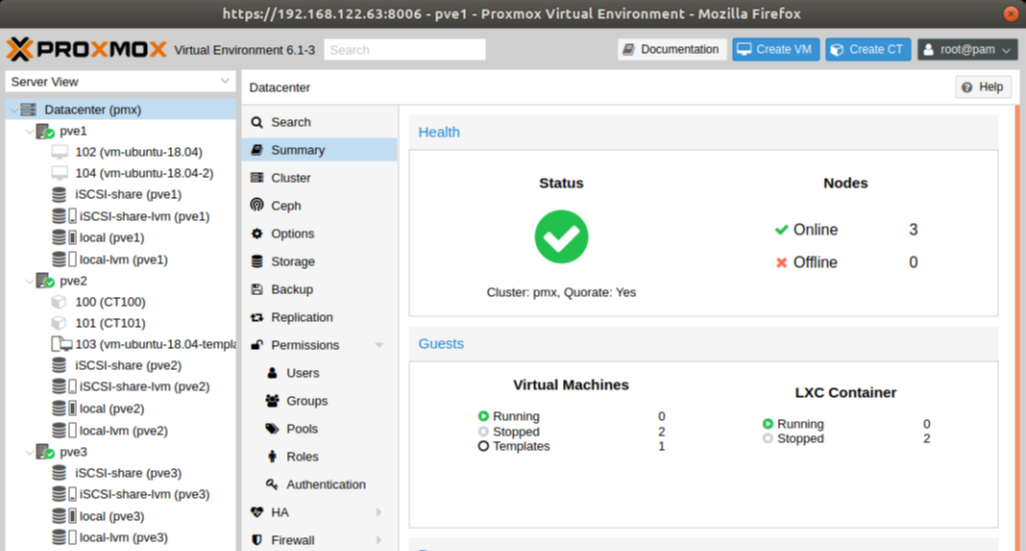
\includegraphics[width=1\textwidth]{9.png}}\\ 
    \label{framework} 
\end{figure}

В качестве гипервизоров могут быть задействованы либо KVM для запуска полноценных виртуальных
машин, либо LXC для запуска Linux-контейнеров. Пользователь может использовать наиболее
подходящую систему виртуализации: полноценную или системные контейнеры. Касательно
возможности использования контейнеров хочется отметить несколько моментов:
\begin{enumerate}
    \item Система виртуализации VMware принципиально не поддерживает запуск контейнеров.
    \item Proxmox, будучи ориентированным на виртуализацию полной системы, не поддерживает
    популярный формат контейнеров приложений. То есть запустить контейнеры Docker не
    получится.
    \item При большей эффективности использования ресурсов хозяйской системы, к сожалению,
    LXC-контейнеры не поддерживают некоторые удобные возможности, такие как живая
    миграция.
\end{enumerate}

Поскольку под капотом Proxmox используются хорошо известные гипервизоры KVM и LXC,
возможности запуска ВМ или виртуальных окружений и управления ими ограничиваются
возможностями соответствующих инструментов. Виртуальное окружение — более корректное
обобщение ВМ и системных контейнеров, поскольку системный контейнер формально нельзя назвать
полноценной ВМ. Если веб-интерфейс Proxmox не даёт возможности задать какие-то особенные
настройки KVM, то данные настройки можно сделать, отредактировав файлы конфигурации KVM на
локальной файловой системе узлов кластера Proxmox.\\

Строго говоря, LXC, как мы помним,— не гипервизор. Однако в данном случае мы используем термин
«гипервизор» для обозначения инструмента управления жизненным циклом ВМ, то есть созданием,
запуском и т. д., оставляя за скобками особенности runtime (времени выполнения).\\

Даже официальное руководство Proxmox предупреждает пользователя, что некоторые операции
невозможно выполнить из графического интерфейса пользователя (веб-интерфейса) и следует
использовать текстовую консоль управления. Получить доступ к консоли управления возможно,
подключившись к данному узлу по SSH или открыв новое окно в веб-браузере. Для этого нужно
нажать на кнопку \textbf{>\_ Shell}, предварительно выбрав необходимый узел. Впрочем, достаточно большое
количество основных операций можно выполнить из веб-интерфейса.\\

Стоит упомянуть следующие возможности Proxmox по управлению виртуальными окружениями в
масштабах кластера:
\begin{enumerate}
    \item Создание виртуальных окружений в полностью ручном режиме и из заранее подготовленных
    шаблонов.
    \item Создание снимков виртуальных окружений из работающих окружений, а также управление
    снимками.
    \item Перенос виртуальных окружений с одного узла кластера на другой. Причём в случае ВМ
    возможен перенос ВМ без её остановки — так называемая live migration. Контейнеры же
    можно перенести только после их остановки.
    \item Создание групп узлов, обеспечивающих высокую доступность (High Availability) виртуальных
    окружений.
\end{enumerate}
\vspace{0.35cm}

По сравнению с предложением VMware есть у Proxmox и некоторые недостатки:
\begin{enumerate}
    \item На момент написания данного материала в Proxmox версии 6.1 всё ещё не реализована
    поддержка динамического распределения ВМ по узлам кластера для балансировки нагрузки.
    В своём \href{https://lists.proxmox.com/pipermail/pve-devel/2019-May/037173.html}{списке рассылки} разработчики Proxmox продолжают обсуждать возможные
    реализации, но пока не принято решение, когда и как это сделать.
    \item Также нет режима, эквивалентного VMware Fault Tolerance, при котором возможно
    продолжение работы ВМ без перезагрузки на другом узле при выходе из строя первого.
\end{enumerate}

Тем не менее Proxmox доступен как для ознакомления, так и для использования в «боевых» системах
совершенно бесплатно, в отличие от таких продуктов, как VMware vCenter Server. Начинающих
пользователей может ввести в заблуждение появляющееся после каждой загрузки Proxmox
сообщение: You do not have a valid subscription for this server («У вас нет действующей подписки для
данного сервера»). Однако оно лишь служит для напоминания о том, что можно купить \href{https://pve.proxmox.com/wiki/Subscriptions}{платную
подписку} (существует несколько вариантов). Таким образом можно получить не только доступ к
репозиториям с ещё более «стабильными» пакетами, но и возможность создавать отчёты об ошибках,
а также поддержать команду разработчиков и мотивировать их продолжать поддерживать и развивать
свой проект.

\subsection*{Настольная лаборатория с Proxmox} 
\addcontentsline{toc}{subsection}{Настольная лаборатория с Proxmox}

В современных реалиях возможно получить опыт работы с вычислительным кластером без
существенных затрат на аппаратуру и ПО. Ниже мы покажем, как создать действующую модель
полноценного вычислительного кластера, чтобы получить на нём опыт реальной работы с
современными системами виртуализации. Причём предложенная реализация будет использовать
почти все технологии, рассмотренные нами на предыдущих занятиях: виртуальные машины,
контейнеры, вложенную виртуализацию.\\

Стоит понимать, что аппаратура, скорее всего, не окажется бесплатной. Однако речь идёт о том, что
затраты на построение полноценного кластера из нескольких серверов, скорее всего, оказались бы
гораздо более существенными, чем использование одной более-менее современной настольной
машины или даже ноутбука.\\

Для начала мы рассмотрим архитектуру полной системы, которую мы будем моделировать. Поскольку
речь идёт о кластере, нам потребуется не один сервер, а несколько. Можно было бы ограничиться
двумя машинами, однако это не даст нам возможности легко реализовать высокую доступность ВМ
(High Availability). Таким образом, нам потребуется три сервера. В самом простом варианте можно
было бы использовать локальный накопитель данных (HDD/SSD) каждого сервера, но это ограничит
нас в возможностях. Для реализации живой миграции, равно как и высокой доступности ВМ,
необходимо вынести накопитель с файловыми системами гостей на внешнее устройство, одинаково
доступное всем серверам. Самое простое решение состоит в использовании сетевого блочного
устройства — по сути, диска, доступного по сети. И тут самое простое решение — это
iSCSI-накопитель.\\

\href{https://ru.wikipedia.org/wiki/ISCSI}{\underbar{\textbf{iSCSI}}} (англ. Internet Small Computer System Interface) — протокол, который базируется на TCP/IP и
разработан для установления взаимодействия и управления системами хранения данных, серверами
и клиентами.\\

Можно либо использовать имеющееся подобное устройство в сети (многие NAS), либо создать такое
устройство самостоятельно на любом компьютере, подключённом к сети.\\

\href{https://ru.wikipedia.org/wiki/NAS}{\underbar{\textbf{NAS}}} (англ. Network Attached Storage) — сервер для хранения данных на файловом уровне. По сути,
представляет собой компьютер с некоторым дисковым массивом, подключённый к сети (обычно
локальной) и поддерживающий работу по принятым в ней протоколам.\\

В итоге мы получим что-то похожее на блок-схему ниже:

\begin{figure}[h]
    \centering
    \scalebox{0.9}{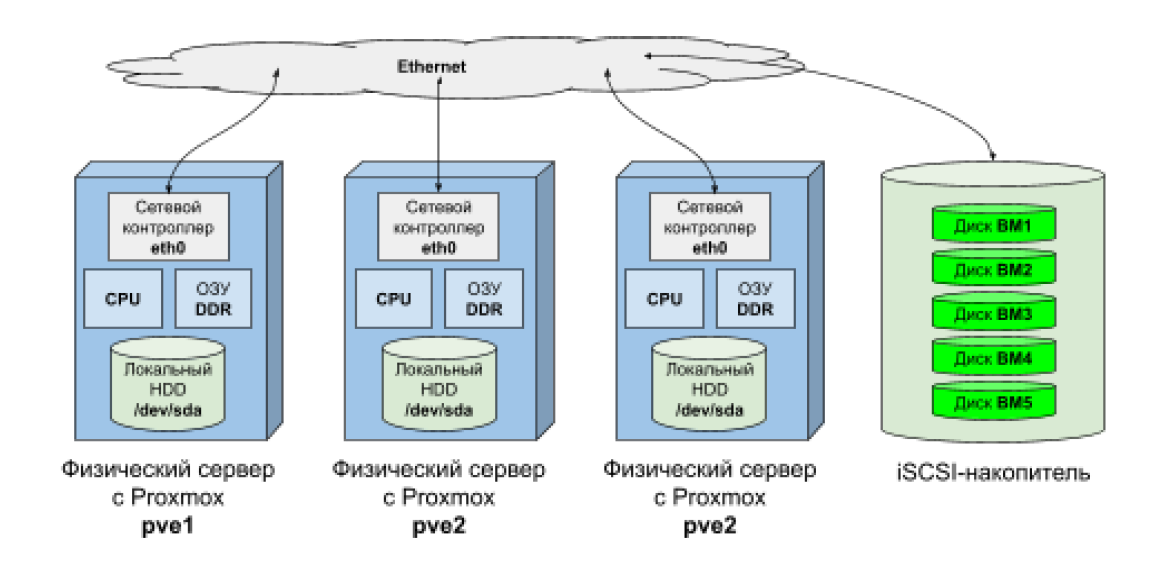
\includegraphics[width=1\textwidth]{10.png}}\\ 
    \label{framework} 
\end{figure}

Поскольку сетевой накопитель данных в системе уже предусмотрен, мы можем отказаться от
использования локальных накопителей на серверах, тем самым несколько упростив общую
архитектуру. В результате мы получим следующую картину:

\begin{figure}[h]
    \centering
    \scalebox{0.9}{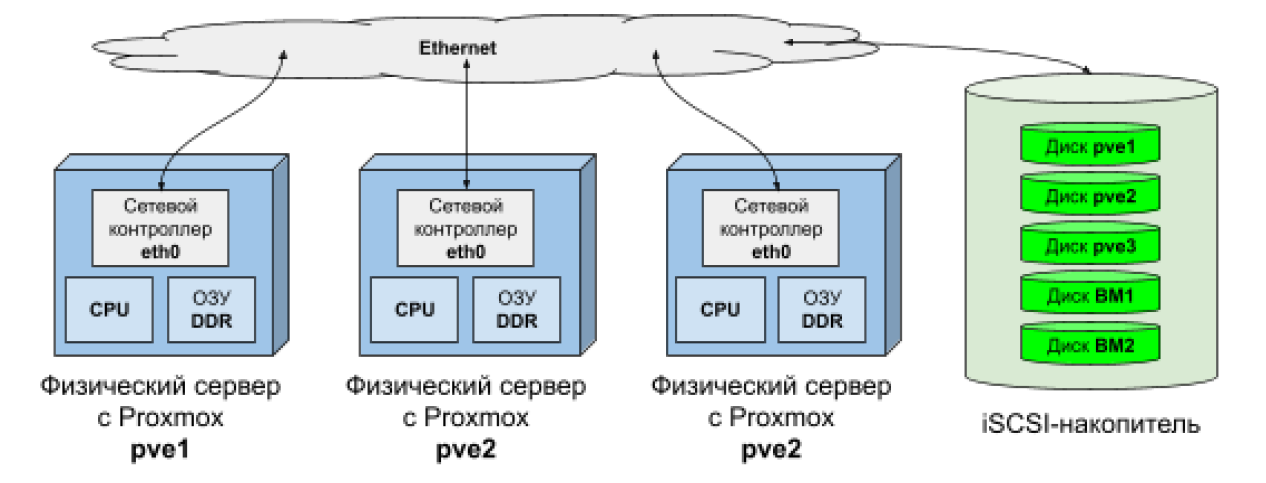
\includegraphics[width=1\textwidth]{11.png}}\\ 
    \label{framework} 
\end{figure}

Как можно видеть, для реализации такой системы нам понадобятся:
\begin{itemize}
    \item три физических машины, каждая из которых поддерживает аппаратную виртуализацию (Intel
    VTx, AMD SVM);
    \item iSCSI-накопитель в сети;
    \item максимально быстро работающая сеть (минимум 1Gb Ethernet).
\end{itemize}

Всё это потребует некоторых инвестиций и определённо займёт достаточно места. Да и управлять
всем этим парком может быть не слишком удобно, особенно в процессе установки основной ОС. На
каждой машине это придётся делать отдельно, имея к ней непосредственный физический доступ.\\

Безусловно, в реальных центрах обработки данных используются специальные
программно-аппаратные комплексы, которые позволяют использовать удалённое подключение
практически для любого вида работ, в том числе и для установки основной ОС. Но мы исходим из
предположения, что у нас нет доступа к такой аппаратуре из-за её баснословной дороговизны.\\

Мы же попробуем собрать и запустить свой лабораторный стенд для изучения современной системы
серверной виртуализации на одной физической машине, используя вложенную виртуализацию. Наша
система будет выглядеть следующим образом:

\newpage

\begin{figure}[h]
    \centering
    \scalebox{0.8}{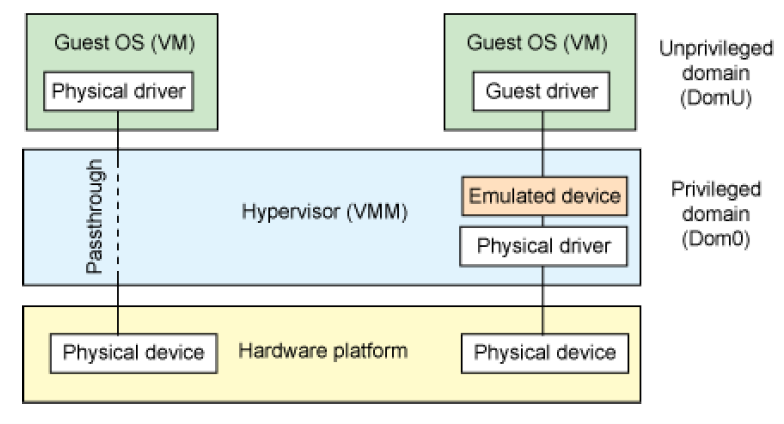
\includegraphics[width=1\textwidth]{12.png}}\\ 
    \label{framework} 
\end{figure}

\subsubsection*{Аппаратура} 
\addcontentsline{toc}{subsubsection}{Аппаратура}

Имея перед глазами архитектуру кластера, можно составить требования к используемой аппаратуре:
\begin{enumerate}
    \item Центральный процессор: 64-битный Intel или AMD с 4 и более ядрами.\\
    
    Intel с поддержкой VT-x и, очень желательно, VT-d и APICv или аналогичное предложение от
    AMD с поддержкой AMD SVM и AMD-Vi. Виртуализация MMU и контроллера прерываний
    позволяет значительно ускорить работу гостевых систем, особенно в случае использования
    вложенной виртуализации. Имеет смысл выделить каждому виртуальному экземпляру
    сервера с Proxmox как минимум по 2 ядра хозяйского процессора. Поскольку мы планируем
    запускать как минимум 3 гостевых системы в гипервизоре первого уровня, то нам желательно
    иметь 3 * 2 = 6 ядер в хозяйском процессоре. Разумеется, можно обойтись и более простым
    хозяйским процессором. Например, 4 ядра, выполняющие по 2 аппаратных потока (Intel
    Hyper-Threading или AMD Simultaneous Multi-Threading).
    \item Оперативная память: 8 Гбайт и более. Желательно 16 Гбайт.\\
    
    \href{https://pve.proxmox.com/wiki/System_Requirements}{Минимальные системные требования для Proxmox VE} на сегодня устанавливают
    минимальный объём ОЗУ 1 Гбайт. У нас будет как минимум 3 таких виртуальных сервера.
    Кроме того, стоит оставить немного ОЗУ для нужд хозяйской системы, то есть потребуется от
    4 Гбайт ОЗУ. Поскольку на виртуальных машинах с Proxmox мы собираемся запускать ещё
    виртуальные машины, которым может потребоваться также от 1 Гбайт ОЗУ, стоит
    предусмотреть возможность выделения 2–4 Гбайт памяти каждому виртуальному серверу с
    Proxmox. В таком случае в хозяйской системе необходимо иметь 8–16 Гбайт ОЗУ.
    \item Место на диске: 100 Гбайт.\\
    
    Каждой виртуальной машине стоит предусмотреть выделение от 10 Гбайт места на диске. Это
    касается и Proxmox-машин, и их гостей. Таких нам будет нужно 5–10 экземпляров.
\end{enumerate}

\subsubsection*{Программное обеспечение} 
\addcontentsline{toc}{subsubsection}{Программное обеспечение}

Разобравшись с аппаратной частью, рассмотрим необходимый набор ПО. Поскольку мы планируем
использовать Proxmox для развёртывания кластера, нам остаётся определиться с тем, что будет
установлено на хозяйскую систему. В теории можно было бы воспользоваться любым современным
гипервизором, который поддерживает вложенную виртуализацию. К таким относятся и VMware ESXi, и
Microsoft Hyper-V, и Xen. Но мы будем использовать KVM как самый легко реализуемый вариант. Мы
же помним, что KVM — это всего лишь загружаемый модуль ядра Linux. То есть весь наш
лабораторный стенд мы сможем собрать в окружении самого обыкновенного Linux-дистрибутива,
сохранив присущие этому дистрибутиву удобства: интернет-браузер, менеджер пакетов, файловый
менеджер и т. д.\\

Нам потребуется следующее ПО:
\begin{enumerate}
    \item Linux-дистрибутив: Ubuntu 18.04.3 LTS, в котором будет использоваться модуль KVM для
    запуска поверх трёх виртуальных узлов вычислительного кластера. Желательно выбирать
    дистрибутивы, использующие ядро Linux версии 5.0, и более свежие. Отлично подойдёт на эту
    роль Ubuntu 18.04.3. Эта рекомендация дана из-за отсутствия необходимости дополнительных
    действий для включения поддержки вложенной виртуализации.
    \item Proxmox, поверх которого мы будем запускать виртуальные машины и LXC-контейнеры и над
    которым мы будем проводить всевозможные эксперименты. Рекомендуется устанавливать
    Proxmox при помощи образа установочного диска. В этом случае можно быть уверенным, что
    не произойдёт конфликтов компонентов и все зависимости будут удовлетворены. Кроме того,
    количество операций, которое нужно выполнить пользователю, сведено к минимуму. Их даже
    меньше, чем при установке любого другого современного Linux-дистрибутива. Это позволяет
    минимизировать вероятность совершения ошибки.
\end{enumerate}

Как мы знаем, Proxmox распространяется совершенно бесплатно в виде образа установочного диска
(.iso) или как набор пакетов для установки в Linux-дистрибутиве Debian, но в любом случае не
существует каких-либо зависимостей от коммерческих продуктов. Интегрированный образ
установщика содержит все необходимые компоненты, так что более ничего устанавливать не
понадобится. Доступна \href{https://pve.proxmox.com/wiki/Installation}{инструкция по установке} 
на английском языке и сами \href{https://www.proxmox.com/en/downloads}{установочные образы}.



\subsubsection*{Создание лабораторного стенда} 
\addcontentsline{toc}{subsubsection}{Создание лабораторного стенда}

\paragraph*{Создание сетевого накопителя iSCSI} \mbox{}\\
\addcontentsline{toc}{paragraph}{Создание сетевого накопителя iSCSI}

Поскольку сетевой накопитель данных потребуется для обеспечения миграции ВМ между серверами
Proxmox, нам придётся его найти или подготовить. Причём даже при наличии этого накопителя в сети
использование iSCSI-накопителя на той же машине, где будут запущены виртуальные сервера,
приведёт к существенному ускорению работы всей системы, так как фактически не будет
использовано медленное сетевое подключение. Даже 10Gb Ethernet существенно уступает в скорости
локальному диску, пусть и с уровнем абстракции поверх него, реализующим виртуальную сеть.\\

Более того, при заранее загруженных на хозяйскую машину дистрибутивах Proxmox и том, что будет
запущено в ВМ и контейнерах поверх Proxmox, можно вообще отключиться от сети обмена данными
(не путать с сетью 220 В) и проводить эксперименты со своим «портативным» кластером даже на
борту самолета. При работе лабораторного стенда будет использоваться достаточно много ресурсов
процессора хозяйской системы, так что не стоит уходить далеко от розетки 220 В.\\

Итак, мы договорились, что на хозяйской системе будет установлен дистрибутив Ubuntu 18.04.3 или
более поздний из семейства 18.04 LTS. Именно для него будут приведены подробные инструкции.
Однако всё то же самое можно повторить и с другим современным Linux-дистрибутивом.\\

Мы договоримся, что строки, начинающиеся с символа \#, — это комментарии, а строки,
начинающиеся с символа \$, — это непосредственно команды, которые необходимо выполнить в
консоли. Причём сам символ \$ вводить не следует. Остальные же строки (без префиксов) — это
реакция системы на введённую выше команду.
\newpage
\begin{lstlisting}
# Установим утилиты для работы с iSCSI-устройством в качестве сервера.
$\textdollar$ sudo apt-get install tgt
    
# Установим утилиты для работы с iSCSI-устройством в качестве клиента.
$\textdollar$ sudo apt-get install open-iscsi
    
# Создаём рабочую директорию.
# Тут будет находиться только образ экспортируемого по сети диска.
$\textdollar$ mkdir -p $\sim$/Projects/virtualization/
    
# Создать пустой образ размером 100 Гбайт.
$\textdollar$ dd if=/dev/zero of=disk.img count=0 bs=1 seek=100G
       
# Создать новый iSCSI-сервер.
$\textdollar$ sudo tgtadm --lld iscsi --op new --mode target --tid 1 -T iqn.com.examp
le:vpe
 
# Подключить новый диск к серверу.
$\textdollar$ sudo tgtadm --lld iscsi --op new --mode logicalunit --tid 1 --lun 1 -b
$\sim$/Projects/virtualization/disk.img
    
# Сделать доступным любым клиентам.
$\textdollar$ sudo tgtadm --lld iscsi --op bind --mode target --tid 1 -I ALL

# Проверить, видны ли экспортированные диски.
$\textdollar$ sudo iscsiadm -m discovery -t sendtargets -p localhost

# Открываем порт 3260 в Firewall для доступа к iSCSI.
$\textdollar$ sudo ufw allow 3260

# Подключаемся к iSCSI-устройству в качестве клиента.
# Это нужно для подготовки диска (LVM) и размещения на нем локальных 
накопителей виртуальных серверов Proxmox.
$\textdollar$ sudo iscsiadm -m node -T iqn.com.example:vpe -p localhost -l

# Проверим, создалась ли сессия.
$\textdollar$ sudo iscsiadm -m session -o show
tcp: [17] 127.0.0.1:3260,1 iqn.com.example:vpe (non-flash)

# Создадим том LVM.
$\textdollar$ sudo pvcreate /dev/sdb
Physical volume "/dev/sdb" successfully created.

# Создадим группу vg_iscsi, которую будем использовать.
$\textdollar$ sudo vgcreate vg_iscsi /dev/sdb
Volume group "vg_iscsi" successfully created
\end{lstlisting}
\vspace{0.2cm}

Теперь наш сетевой диск готов к использованию. Мы можем приступить к созданию виртуальных
серверов с Proxmox.

\paragraph*{Создание виртуальных серверов с Proxmox} \mbox{}\\
\addcontentsline{toc}{paragraph}{Создание виртуальных серверов с Proxmox}

\noindent Для каждого сервера нам необходимо подготовить раздел на сетевом диске, где будет содержаться
корневая файловая система сервера.
\newpage
\begin{lstlisting}
# Создадим раздел "lv_pve1" размером 10 Гбайт в LVM-группе "vg_iscsi"
$\textdollar$ sudo lvcreate -n lv_pve1 -L 10G vg_iscsi
\end{lstlisting}
\vspace{0.2cm}

\noindent Создадим ВМ со следующими параметрами:
\begin{itemize}
    \item название — pve1 (--name=pve1);
    \item 2 виртуальных ядра (--vcpus=2);
    \item процессор такой же, как в хозяйской системе\\
    (--cpu=host-passthrough,cache.mode=passthrough);
    \item 2 Гбайт ОЗУ (--memory=2048);
    \item накопитель размером 10 Гбайт с корневой файловой системой будет расположен в ранее
    созданном разделе lv\_pve1 \\ (- - disk path=/dev/vg\_scsi/lv\_pve1,size=10 );
    \item образ компакт-диска proxmox-ve\_6.1-1.iso с установщиком дистрибутива гостевой ОС
    расположен в папке $\mathtt{\sim}$/Projects/virtualization/isos \\
    (--cdrom=isos/proxmox-ve\_6.1-1.iso).
\end{itemize}
\vspace{0.3cm}

Следующие операции можно было бы выполнить из графического интерфейса Virtual Machine
Manager, но вместо дюжины картинок можно обойтись одной строчкой в командной строке:
\vspace{0.3cm}
\begin{lstlisting}
$\textdollar$ virt-install --name=pve1 --vcpus=2
--cpu=host-passthrough,cache.mode=passthrough --memory=2048 --disk
path=/dev/vg_iscsi/lv_pve1,size=10 --cdrom=isos/proxmox-ve_6.1-1.iso   
\end{lstlisting}
\vspace{0.2cm}

Результатом выполнения последней команды должно стать создание ВМ и её запуск. При этом
должно появиться окно с графическим установщиком Proxmox.

\begin{figure}[h]
    \centering
    \scalebox{0.505}{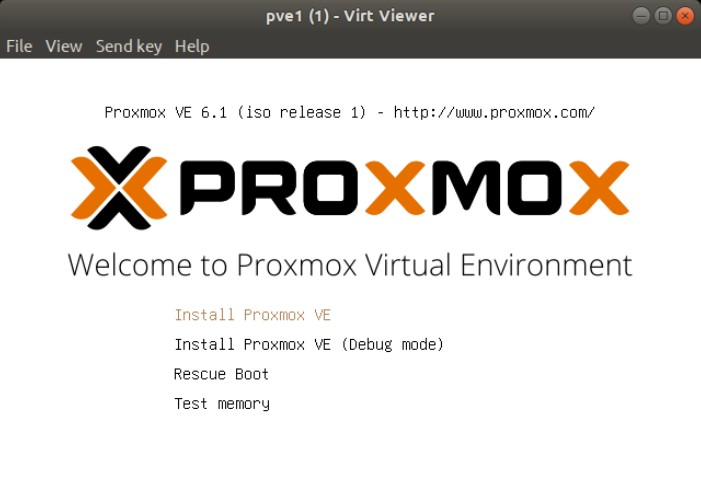
\includegraphics[width=1\textwidth]{13.png}}\\
    \small\textit{Старт установщика Proxmox в виртуальной машине}  
    \label{framework} 
\end{figure}

Теперь можно пройти по шагам процедуру установки Proxmox, перезагрузить ВМ.
\begin{figure}[h]
    \centering
    \scalebox{0.7}{
\includegraphics[width=1\textwidth]{14.png}}\\
    \small\textit{Процедура установки окончена, необходимо перезагрузить ВМ}  
    \label{framework} 
\end{figure}

И войти в графический интерфейс Proxmox из браузера хозяйской системы.

\begin{figure}[h]
    \centering
    \scalebox{0.7}{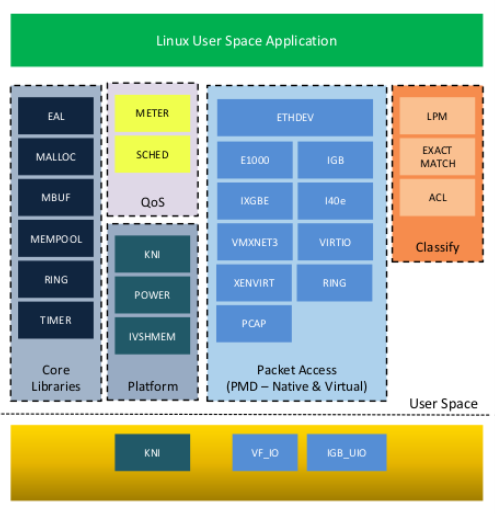
\includegraphics[width=1\textwidth]{15.png}}\\
    \small\textit{Веб-интерфейс управления Proxmox}  
    \label{framework} 
\end{figure}

Итак, первый Proxmox-сервер готов. Осталось повторить ту же процедуру для ещё двух серверов, и
можно будет объединять серверы в кластер.
\vspace{0.15cm}
\begin{lstlisting}
# Создадим разделы "lv_pve2" и "lv_pve3" размером 10 Гбайт в LVM-группе
"vg_iscsi".
$\textdollar$ sudo lvcreate -n lv_pve2 -L 10G vg_iscsi
\end{lstlisting}
\newpage
\begin{lstlisting}
$\textdollar$ sudo lvcreate -n lv_pve3 -L 10G vg_iscsi
   
# Создадим второй сервер Proxmox.
$\textdollar$ virt-install --name=pve2 --vcpus=2
--cpu=host-passthrough,cache.mode=passthrough --memory=2048 --disk
path=/dev/vg_iscsi/lv_pve2,size=10 --cdrom=isos/proxmox-ve_6.1-1.iso

# Создадим третий сервер Proxmox.
$\textdollar$ virt-install --name=pve3 --vcpus=2
--cpu=host-passthrough,cache.mode=passthrough --memory=2048 --disk
path=/dev/vg_iscsi/lv_pve3,size=10 --cdrom=isos/proxmox-ve_6.1-1.iso
\end{lstlisting}
\vspace{0.2cm}

Готовые узлы (виртуальные серверы Proxmox) легко вводятся в кластер, если следовать инструкциям
в соответствующей \href{https://pve.proxmox.com/wiki/Cluster_Manager#pvecm_join_node_to_cluster}{статье «Википедии» Proxmox}.\\

Важное замечание, которое есть в статье, указанной выше: очень скоро после начала вхождения в
кластер вводимый туда узел изменит свой сертификат, используемый для установления защищённого
HTTPS-соединения, на сертификат кластера, а потому сессия в браузере окажется недействительной.
При желании можно перезагрузить веб-страницу и заново войти в интерфейс. На самом деле нет
необходимости иметь доступ к веб-интерфейсу всех узлов, введённых в кластер, так как управление
ими можно осуществлять из веб-интерфейса любого узла.\\


\begin{figure}[h]
    \centering
    \scalebox{0.8}{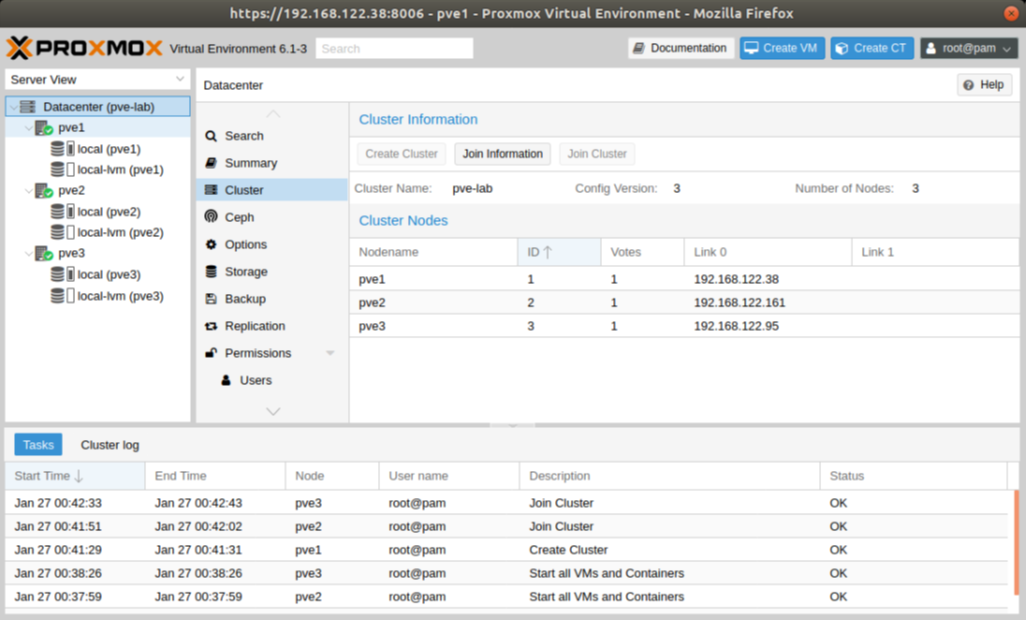
\includegraphics[width=1\textwidth]{16.png}}\\
    \small\textit{Кластер из трёх виртуальных серверов Proxmox}  
    \label{framework} 
\end{figure}

В таком кластере можно уже устанавливать и запускать контейнеры и ВМ, но без внешнего диска не
получится попробовать миграцию. Тогда мы подключим ранее подготовленный iSCSI-диск.
\newpage
\begin{figure}[h]
    \centering
    \scalebox{0.8}{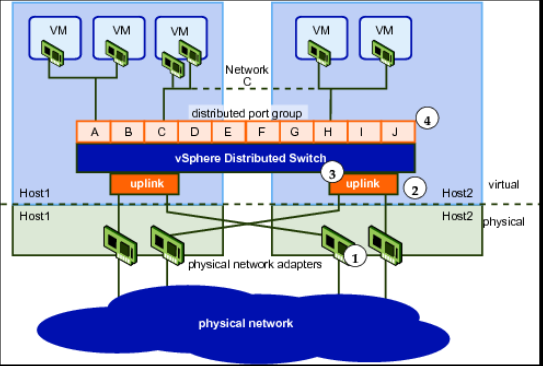
\includegraphics[width=1\textwidth]{17.png}}\\
    \label{framework} 
\end{figure}


Добавим iSCSI-устройство. В поле Portal необходимо указать адрес хозяйской системы в подсети
виртуальных машин. Его можно посмотреть у сетевого моста, используемого KVM:
\vspace{0.3cm}
\begin{lstlisting}
$\textdollar$ ip -4 addr show virbr0
4: virbr0: <BROADCAST,MULTICAST,UP,LOWER_UP> mtu 1500 qdisc noqueue state 
UP
group default qlen 1000
    inet $\mathbf{192.168.122.1}$/24 brd 192.168.122.255 scope global virbr0
    valid_lft forever preferred_lft forever
\end{lstlisting}
\vspace{0.2cm}

В выпадающем меню Target нужно выбрать название сервера iSCSI (iqn.com.example:vpe), которое мы
задали при его создании.

\begin{figure}[h]
    \centering
    \scalebox{0.6}{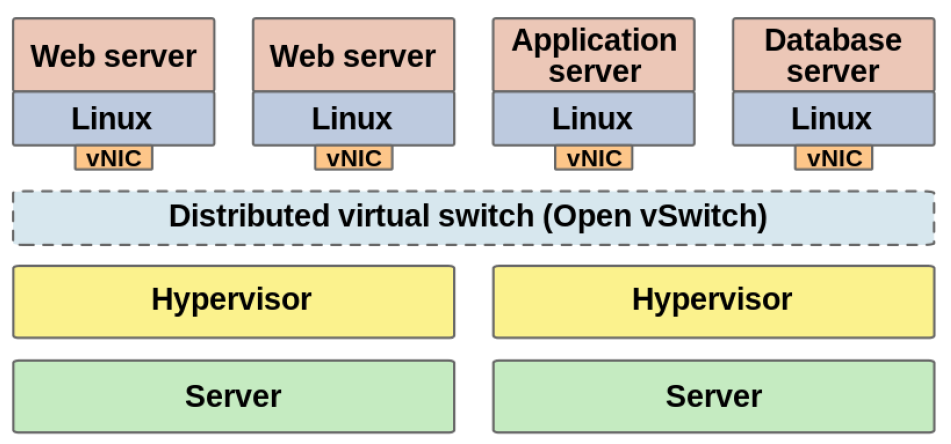
\includegraphics[width=1\textwidth]{18.png}}\\
    \label{framework} 
\end{figure}

Затем добавим накопитель с LVM. Именно его мы будем использовать для установки контейнеров и
ВМ в окружении Proxmox. Нам нужно выбрать в выпадающем меню только группу LVM-томов
(vg\_iscsi), которую мы создали на внешнем диске ранее.

\newpage

\begin{figure}[h]
    \centering
    \scalebox{0.6}{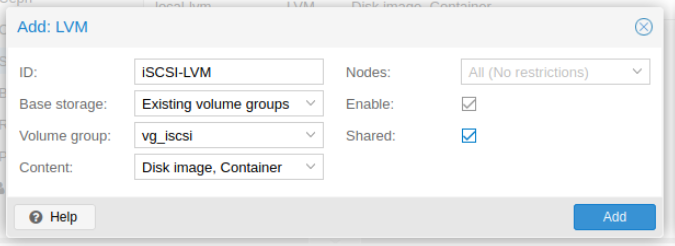
\includegraphics[width=1\textwidth]{19.png}}\\
    \label{framework} 
\end{figure}

Сетевой диск готов к работе!

\begin{figure}[h]
    \centering
    \scalebox{0.8}{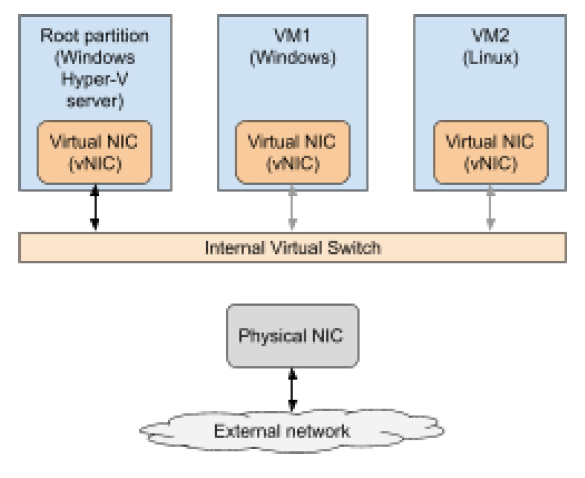
\includegraphics[width=1\textwidth]{20.png}}\\
    \label{framework} 
\end{figure}

Можно обратить внимание, что 30\%, то есть 30 Гбайт, диска iSCSI-LVM уже занято. Это как раз
образы файловых систем Proxmox-серверов.

\paragraph*{Создание виртуальной машины} \mbox{}\\
\addcontentsline{toc}{paragraph}{Создание виртуальной машины}

Поскольку наша задача сейчас состоит в изучении системы управления виртуализацией, а не в
запуске сложных задач внутри целевых ВМ, мы можем позволить себе использовать для
экспериментов минималистичные ВМ. Например,\href{https://help.ubuntu.com/community/Installation/MinimalCD}{ Ubuntu Server из netinstall-образа}.\\

Важно понимать, что небольшой размер образа с установщиком ОС обусловлен отсутствием
реальных пакетов, которые будут установлены в целевую систему: они во время установки будут
загружены из сети. Если желательно избежать загрузки дополнительных пакетов по сети, например,
сеть может оказаться недоступна в момент установки ВМ, то следует использовать образ с 
\href{https://ubuntu.com/download/server}{полным установщиком}.\\

Образ компакт-диска необходимо загрузить на «локальный» накопитель одного из Proxmox-серверов.

\begin{figure}[h]
    \centering
    \scalebox{1}{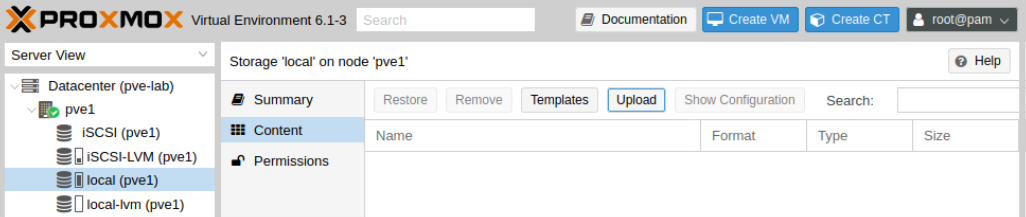
\includegraphics[width=1\textwidth]{21.png}}\\
    \small\textit{Кнопка диалога для загрузки файлов на локальное хранилище Proxmox-сервера}  
    \label{framework} 
\end{figure}

\begin{figure}[h]
    \centering
    \scalebox{1}{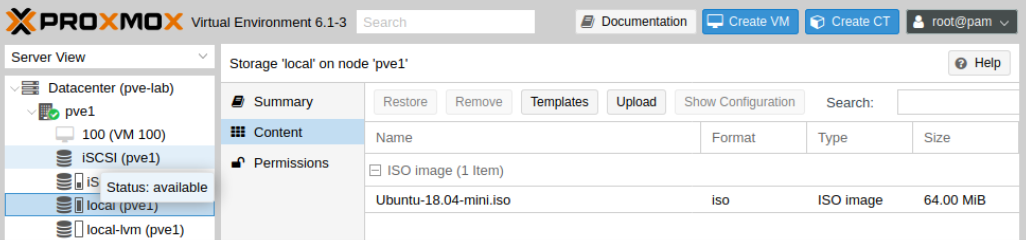
\includegraphics[width=1\textwidth]{22.png}}\\
    \small\textit{Загруженный образ установщика Linux-дистрибутива на локальном хранилище Proxmox-сервера}  
    \label{framework} 
\end{figure}

После этого можно приступить к созданию первой виртуальной машины. При её создании важно
указать ранее загруженный образ компакт-диска как источник установщика ОС, а также выбрать в
качестве накопителя сетевой диск. Причём выбирать нужно не само iSCSI-устройство, а накопитель с
томами LVM (iSCSI-LVM).

\begin{figure}[h]
    \centering
    \scalebox{0.7}{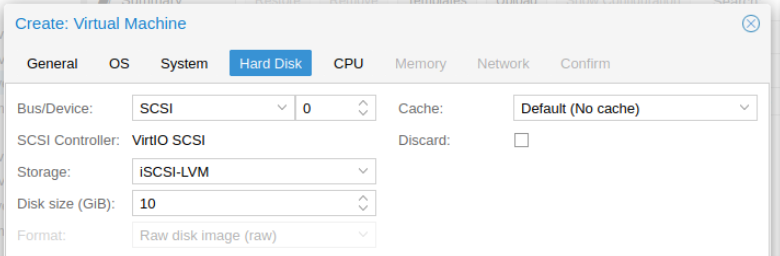
\includegraphics[width=1\textwidth]{23.png}}\\
    \small\textit{Выбор накопителя для размещения основной файловой системы создаваемой ВМ}  
    \label{framework} 
\end{figure}

С контейнерами дело обстоит ещё проще. Proxmox предоставляет набор шаблонов (templates) для
создания контейнеров из самых популярных Linux-дистрибутивов. Достаточно просто выбрать что-то
на свой вкус и загрузить на локальный диск Proxmox-сервера.

\newpage

\begin{figure}[h]
    \centering
    \scalebox{1}{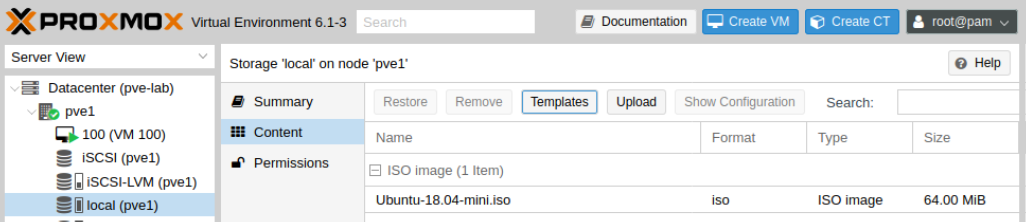
\includegraphics[width=1\textwidth]{24.png}}\\
    \small\textit{Кнопка для перехода к панели управления шаблонами LXC-контейнеров в Proxmox}  
    \label{framework} 
\end{figure}

\begin{figure}[h]
    \centering
    \scalebox{0.7}{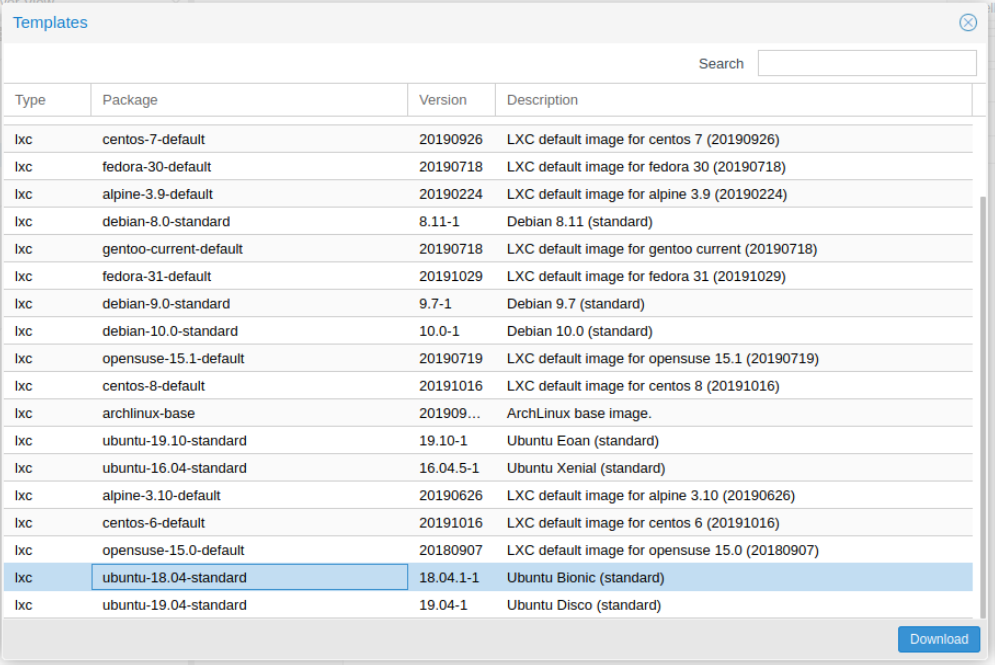
\includegraphics[width=1\textwidth]{25.png}}\\
    \small\textit{Доступные для выбора шаблоны LXC-контейнеров в Proxmox}  
    \label{framework} 
\end{figure}

Однако при желании можно использовать и \href{https://uk.lxd.images.canonical.com/images/}{любой другой образ LXC-контейнера}.\\

После создания нескольких экземпляров ВМ и/или контейнеров можно провести эксперименты:

\begin{itemize}
    \item мигрировать ВМ и контейнер с одного сервера Proxmox на другой;
    \item создать снимок ВМ или контейнера;
    \item создать шаблон ВМ или контейнера.
\end{itemize}

Рассмотрим подробнее, как переместить ВМ и контейнер. Зная IP-адрес перемещаемой ВМ или
контейнера, можно запустить утилиту ping на хозяйской системе и понаблюдать, будет ли
перемещаемая ВМ или контейнер отвечать во время и после перемещения. Чтобы узнать IP-адрес,
достаточно выполнить команду \colorbox{backcolour}{ip addr} внутри ВМ или контейнера.\\

Нужно пометить ВМ или контейнер как HA (High Availability) объект:

\begin{figure}[h]
    \centering
    \scalebox{1}{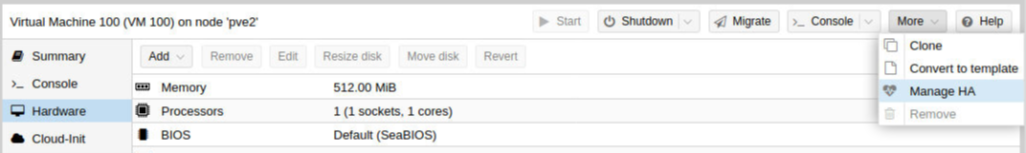
\includegraphics[width=1\textwidth]{26.png}}\\  
    \label{framework} 
\end{figure}

\begin{figure}[h]
    \centering
    \scalebox{0.7}{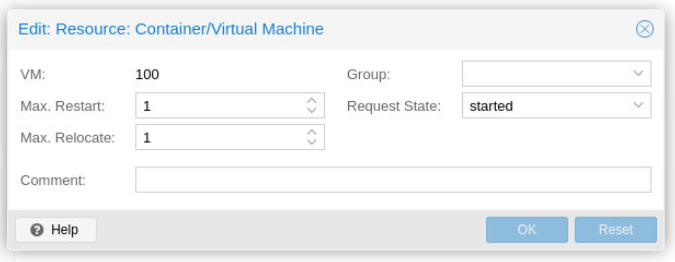
\includegraphics[width=1\textwidth]{27.png}}\\  
    \label{framework} 
\end{figure}

После этого можно сымитировать выход из строя Proxmox-сервера, на котором в настоящий момент
выполняется данный гость. Для этого в интерфейсе управления виртуальными машинами хозяйской
системы (Virtual Machine Manager) принудительно остановите соответствующий виртуальный
Proxmox-сервер.

% \begin{figure}[h]
%     \centering
%     \scalebox{0.6}{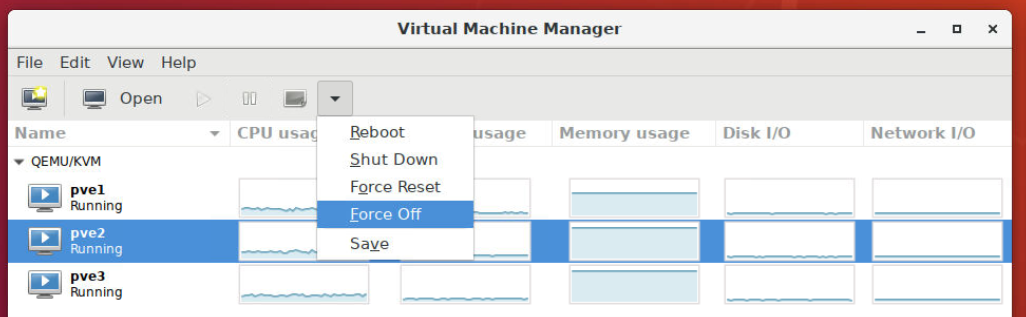
\includegraphics[width=1\textwidth]{28.png}}\\ 
%     \small\textit{Отключение одного из виртуальных серверов Proxmox}  
%     \label{framework} 
% \end{figure}

\begin{figure}[h]
    \centering
    \scalebox{0.8}{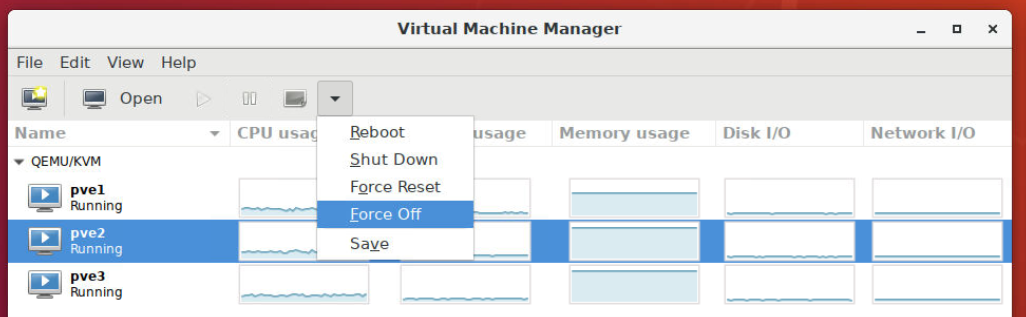
\includegraphics[width=1\textwidth]{28.png}}\\ 
    \small\textit{Отключение одного из виртуальных серверов Proxmox}\\
    \vspace{0.5cm}
    \scalebox{0.19}{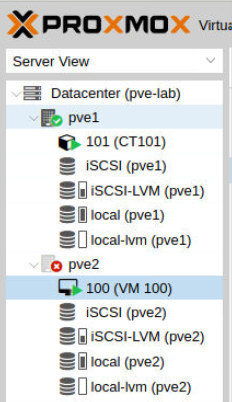
\includegraphics[width=1\textwidth]{29.png}}
    \scalebox{0.8}{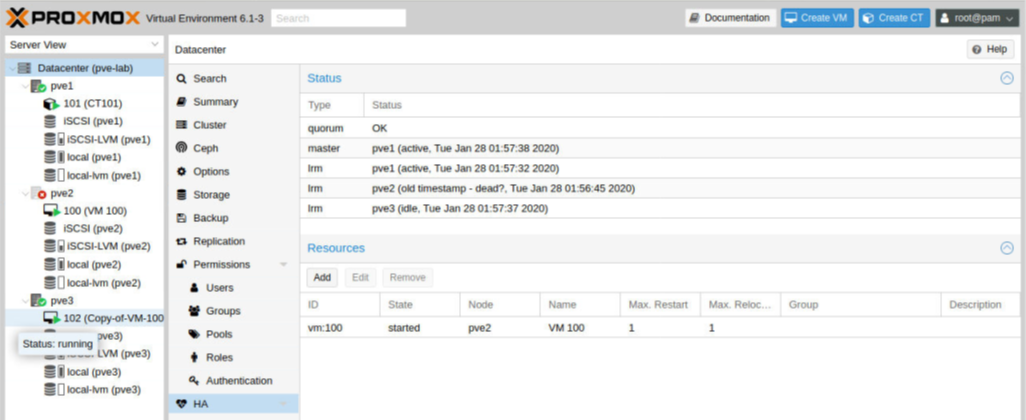
\includegraphics[width=1\textwidth]{30.png}}\\ 
    \small\textit{Перезапуск ВМ на работающем узле кластера}  
    \label{framework} 
\end{figure}

Примерно через две минуты ВМ окажется снова запущена, но уже на другом сервере. Реакция на
потерю связи с узлом умышленно выполняется с ощутимой задержкой для избежания ситуаций, когда
связь может восстановиться и работа кластера может оказаться нарушенной: появится узел, который
другие узлы уже не ожидали увидеть. Подробности можно прочитать в 
\href{https://pve.proxmox.com/pve-docs/pve-admin-guide.html#chapter_ha_manager}{руководстве по администрированию}.\\

Интересно отметить, что Proxmox позволяет гибко настраивать политику управления HA-ресурсами.
Например, можно потребовать перемещать ресурс на другие серверы с определённой очерёдностью.
По умолчанию, когда не выбраны приоритеты, миграция происходит на любой из работающих узлов.\\

Всё перечисленное выше — это лишь базовые возможности, предоставляемые Proxmox. Кроме того,
Proxmox поддерживает использование ZFS и CEPH.\\

\href{https://ru.wikipedia.org/wiki/ZFS}{\underbar{\textbf{ZFS}}} (Zettabyte File System) — файловая система, изначально созданная в Sun Microsystems для
операционной системы Solaris. В настоящее время становится весьма популярной в системах
хранения данных, поскольку считается, что она обеспечивает исключительно высокую надёжность
сохранения данных, поддерживая их целостность.

\href{https://ru.wikipedia.org/wiki/Ceph}{\underbar{\textbf{Ceph}}} — свободная программная объектная сеть хранения (англ. object storage), обеспечивающая как
файловый, так и блочный интерфейсы доступа. По сути, отказоустойчивое распределённое
хранилище данных, работающее по протоколу TCP.\\

Для гибкого управления сетью и маршрутизацией пакетов данных может быть использован Open
vSwitch. С более полным списком особенностей Proxmox можно ознакомиться в \href{https://www.proxmox.com/en/proxmox-ve/features}{соответствующем
разделе веб-сайта проекта}.

\subsection*{oVirt} 
\addcontentsline{toc}{subsection}{oVirt}

Ранее мы рассмотрели Proxmox как достаточно простой в освоении и использовании инструмент для
управления виртуализованной инфраструктурой. Но помимо него на рынке существуют и другие
решения с открытым исходным кодом. В частности, oVirt, разработка которого спонсируется
компанией Red Hat (ныне это часть IBM). По сути, oVirt — будущая версия Red Hat Virtualization в том
же смысле, как и Linux-дистрибутив Fedora используется инженерами Red Hat для обкатки новых
технологий. Некоторая версия Fedora впоследствии станет основой для очередного выпуска Red Hat
Enterprise Linux. Red Hat Virtualization, в свою очередь, преподносится как альтернатива VMware
vSphere.\\

oVirt, как и Proxmox, использует гипервизор KVM, поддерживает разнообразные файловые системы и
накопители: GlusterFS, NFS, iSCSI и т. д.\\

\href{https://ru.wikipedia.org/wiki/GlusterFS}{\underbar{\textbf{GlusterFS}}} — это распределённая, параллельная, линейно масштабируемая файловая система с
возможностью защиты от сбоев.\\

\href{https://ru.wikipedia.org/wiki/Network_File_System}{\underbar{\textbf{Network File System}}} (NFS) — протокол сетевого доступа к файловым системам. Первоначально
разработан Sun Microsystems в 1984 году. Позволяет подключать (монтировать) удалённые файловые
системы через сеть.\\

В состав oVirt входит два типа объектов: узлы (nodes), то есть серверы с CentOS/Fedora или
специально подготовленным Linux-дистрибутивом oVirt Node, а также Engine — сервер,
координирующий работу узлов oVirt-инфраструктуры. И, соответственно, минимальный состав
системы включает в себя один узел и один Engine.\\

\href{https://www.ovirt.org/download/node.html}{\underbar{\textbf{oVirt Node}}} — это минималистичная ОС, основанная на CentOS, предназначенная для работы в
качестве одного из узлов oVirt.\\

oVirt Engine чем-то сильно напоминает VMware vCenter Server. Интересно, что в отличие от продуктов
VMware vSphere и oVirt, в ProxMox управление кластером можно осуществлять с любого узла.

\begin{figure}[h]
    \centering
    \scalebox{0.8}{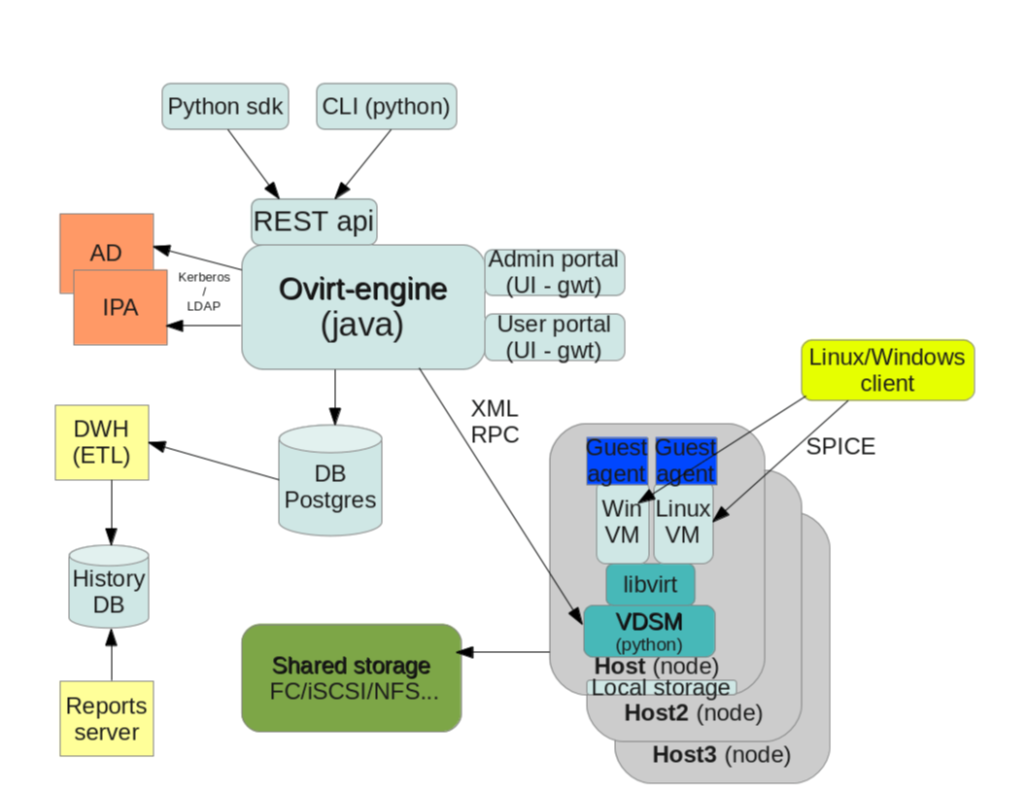
\includegraphics[width=1\textwidth]{31.png}}\\ 
    \small\textit{\href{https://www.ovirt.org/develop/architecture/architecture.html}{Архитектура oVirt}}  
    \label{framework} 
\end{figure}

\newpage

\begin{figure}[h]
    \centering
    \scalebox{1}{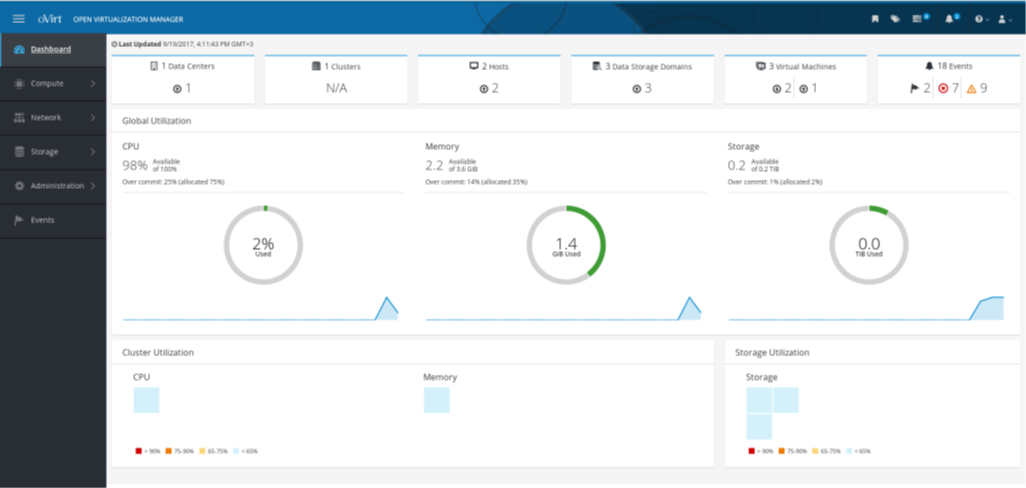
\includegraphics[width=1\textwidth]{32.png}}\\ 
    \small\textit{Веб-интерфейс управления oVirt}  
    \label{framework} 
\end{figure}

При том, что на первый взгляд oVirt мало чем отличается от Proxmox, она считается более
подходящим решением для сложных систем с большим количеством узлов. Возможно, это связано с
основным спонсором — компанией RedHat, которая не только выделяет ресурсы своих инженеров
для работы над oVirt и гипервизором KVM, но также всячески продвигает это решение среди своих
клиентов, а также в сообществе разработчиков ПО с открытым исходным кодом.\\

Тем не менее любой желающий может ознакомиться с \href{https://www.ovirt.org/documentation/}{документацией} и поэкспериментировать с oVirt,
так как все \href{https://www.ovirt.org/download/}{компоненты} доступны для свободной загрузки и использования.

\section*{Заключение} 
\addcontentsline{toc}{section}{Заключение}

В этом курсе мы рассмотрели разнообразные аспекты систем виртуализации, начиная с истории
становления технологий виртуализации и заканчивая современными системами управления
виртуализованной инфраструктурой. Надеемся, что эти знания помогут вам более эффективно
решать задачи, связанные с разработкой, развёртыванием и поддержкой систем и сервисов,
полагающихся на использование виртуализованных окружений разного рода: контейнеров
приложений или полноценных виртуальных машин.

\newpage

\section*{Практическое задание} 
\addcontentsline{toc}{section}{Практическое задание}

\begin{enumerate}
    \item * Установите кластер из трёх виртуальных серверов Proxmox и выполните миграцию ВМ и
    контейнера с одного виртуального сервера на другой.
    \item Перечислите преимущества вычислительного кластера перед одной, но более мощной
    машиной или несколькими независимыми серверами.
    \item Назовите преимущества использования виртуальных машин поверх кластера из нескольких
    серверов.
\end{enumerate}

\section*{Используемые источники} 
\addcontentsline{toc}{section}{Используемые источники}

\begin{enumerate}
    \item \href{https://www.amazon.com/Mastering-VMware-vSphere-Nick-Marshall/dp/1119512948}{\textit{Mastering VMware vSphere 6.7.}}
    \item \href{https://www.amazon.com/VMware-vSphere-6-7-Cookbook-orchestrate/dp/1789953006}{\textit{VMware vSphere 6.7 Cookbook.}}
    \item \href{https://docs.vmware.com/en/VMware-vSphere/index.html}{\textit{VMware vSphere Documentation}}.
    \item \href{https://medium.com/@alexander.bazhenov/установка-vmware-vcenter-server-appliance-5beb779ff2c3}{\textit{Установка VMware vCenter Server Appliance и создание кластера vSphere}}.
    \item \href{https://www.usenix.org/legacy/event/nsdi08/tech/full_papers/cully/cully_html/index.html}{\textit{Remus: High Availability via Asynchronous Virtual Machine Replication}}.
    \item \href{https://www.vmgu.ru/ext/books/vsphere-ha-deepdive.pdf}{\textit{VMware vSphere 6.x HA Deepdive}}.
    \item \href{https://www.packtpub.com/product/mastering-proxmox-second-edition/9781785888243}{\textit{Mastering Proxmox - Third Edition}}.
    \item \href{http://onreader.mdl.ru/MasteringProxmox.3ed/content/index.html}{\textit{Proxmox. Полное руководство}}.
    \item \href{https://subscription.packtpub.com/search?query=getting%20started%20ovirt%2033}{\textit{Getting Started with oVirt 3.3}}.
\end{enumerate}


\end{document}